The overview of Bluetooth Hydrometer is provided in this section. Arduino Nano 33 BLE is a microcontroller used for Bluetooth Hydrometer. Nano 33 is a small and low powered Bluetooth enabled device with a built in 9-axis gyroscope. Nano operates at 3.3 V, it has 14 digital inputs, 8 analog inputs and 6 power modulations (PWM) and a clock speed of 64 MHz. Temperature sensor used operates at 3.3V with temperature range of $-$40 to 125$^\circ$C having an accuracy of  $\pm$1.5$^\circ$C.

\begin{figure}[h!]
	\centering
   	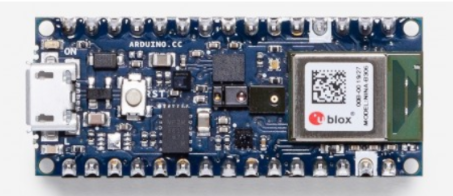
\includegraphics[width=0.60\textwidth]{images/arduino_nano_33}
    \caption{Arduino Nano 33}
\end{figure}
\begin{figure}[h!]
	\centering
   	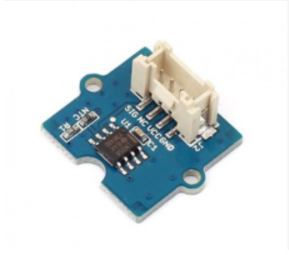
\includegraphics[width=0.60\textwidth]{images/temperature_sensor}
    \caption{Temperature Sensor}
\end{figure}

\subsection{Features \& Functions}
What the product does and does not do. Specify in words what it looks like, referring to a conceptual diagram/graphic (Figure X).  Define the principle parts/components of the product. Specify the elements in the diagram/graphic that are part(s) of this product as well as any associated external elements (e.g., the Internet, an external web server, a GPS satellite, etc.)

\subsection{External Inputs \& Outputs}
External input is temperature and specific gravity data from temperature sensor and built in gyroscope sensor respectively. Arduino nano outputs those data to smartphones via Bluetooth and a website.

\subsection{Product Interfaces}
Bluetooth module plays an important role to interface nano. Datas are constantly uploaded via Bluetooth to a smartphone or a website. Nano can be interfaced  to send data only after a certain time interval, since temperature and SG don't change every second or minute. Software can handle and analyze those datas within an app or a website to provide visual interface to users.
